\subsection{Algoritmo de simplificación por herencia vertical}
	\label{sec:vertical}
	% Autoridad > derecho limitado a una porcion
	% Claridad > autoridad no ambigua
	% Anticipacion > avisar con antelacion
	% Granularidad > rutas cortas y funcionales
	% Terminalidad > avisar fin de via
	% Infraestructura > avisar de infraestructura
	% No bloqueo > circulacion fluida
	
	Como se explicó en la Sección \ref{sec:switches}, una máquina de cambios bifurca la vía principal en dos: una vía que continúa la rama principal y otra vía que se convierte en una rama secundaria. Tanto la vía de continuación como la vía ramificada pueden tener otra máquina de cambios que, a su vez, vuelve a dividir el trazado ferroviario en dos. Esto incrementa más y más el nivel de complejidad de la red, añadiendo caminos divergentes al principal que luego, mas adelante, podrían, o no, volver a converger utilizando mas máquinas de cambios. Cada divergencia aporta un nivel de profundidad a la red, mientras que cada convergencia reduce en uno el nivel de profundidad.
	
	Una máquina de cambios que tiene en cualquiera de sus ramas divergentes el nodo de inicio de otra máquina de cambios a una distancia pequeña es un cambio compuesto. Los cambios compuestos requieren considerar a ambas máquinas de cambios como una sola, ya que es necesario posicionar ambos mecanismos para completar un movimiento. El ejemplo de La Figura \ref{fig:signal_vertical_1} ayudará a clarificar el concepto de cambios compuestos e introducir el Algoritmo de simplificación por herencia vertical.	

	\begin{figure}[h!]
		\centering
		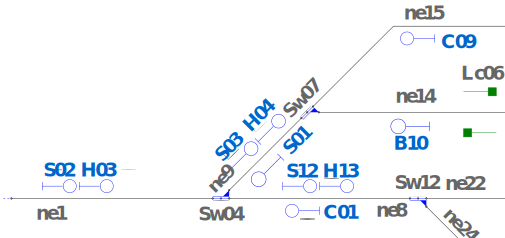
\includegraphics[width=1\textwidth]{Figuras/Figure8_Crop.pdf}
		\centering\caption{Señalamiento generado, simplificado por algoritmo de herencia vertical.}
		\label{fig:signal_vertical_1}
	\end{figure}
	
	En la Sección \ref{sec:signal_switches} se introdujo el Algoritmo \ref{alg:SW} que define la asignación de señalamiento para los cambios de vías: una señal de circulación (S) y de maniobra (H) para el nodo de inicio (S), una señal de circulación para el nodo de continuación (C) y una señal de maniobras para el nodo de desvío (B). El Algoritmo \ref{alg:SW} se aplicó de forma independiente a las máquinas de cambios Sw04, Sw07 y Sw12 y se obtuvo el señalamiento de la Figura \ref{fig:signal_vertical_1}. No obstante, el señalamiento generado no cumple con el principio de no bloqueo, al situar las señales S03, H04, B01, S12, H13 y C01 en las secciones correspondientes a los netElements ne9 y ne8. De esa manera, las formaciones podrían detenerse en esas secciones si las mencionadas señales presentasen un aspecto rojo.
	
	Una formación detenida en la sección correspondiente al netElement ne9 no permitiría mover el cambio de vía Sw04, al tener parte de la formación aún en ne1. Tampoco permitiría accionar el cambio de vías Sw07 al no haber finalizado el movimiento. Análogamente para una formación detenida en la sección correspondiente al netElement ne8. Es necesario que el movimiento finalice, despejando las secciones y permitiendo que otras formaciones utilicen los cambios de vías Sw04 y Sw07, o cualquier combinación de mas de un cambio de vías.
	
	Para solucionar el problema expuesto, el RNA aplica el Algoritmo \ref{alg:vertical} de simplificación por herencia vertical para reposicionar las señales situadas en zonas conflictivas. A diferencia del señalamiento explicado en la Sección \ref{sec:generacion}, las señales que protegen a un cambio de vías B situado en una rama mas profunda de la red no se encuentran inmediatamente precediendo al cambio de vías B. Estas señales son movidas a ramas de menor profundidad con suficiente espacio físico para contenerlas, situándose precediendo a otro cambio de vías A que decimos que ha \emph{heredado} el señalamiento del cambio de vía B.
		
	\begin{algorithm}[hbt!]
        \caption{Algoritmo de simplificación por herencia vertical}\label{alg:vertical}
        \DontPrintSemicolon
        %\SetAlgoLined
        \SetNoFillComment
        \LinesNotNumbered 
        \For{ each Signal protecting a Sw\_A }
        {
            \For{each Sw\_B != Sw\_A}
            {
                \tcc{Criteria \#0}
                \If{distance(Sw\_A,Sw\_B) $>$ MIN\_DISTANCE}
                {
                    Continue\;
                }
                \If{S in Sw\_A.Branch also in Sw\_B.Start} 
                {
                   \tcc{Criteria \#1}
                   \If{S points to Sw\_B.Start}
                   {
                        Move S to Sw\_A.Start\;
                   }
                   \tcc{Criteria \#2}
                   \If{S points to Sw\_A.Branch}
                   {
                        Move S to Sw\_B.Continue\;
                        Move S to Sw\_B.Branch\;
                   }
                }
                \If{S in Sw\_A.Continue also in Sw\_B.Start}
                {
                   \tcc{Criteria \#3}
                   \If{S points to Sw\_B.Start}
                   {
                        Move S to Sw\_A.Start\;
                   }
                   \tcc{Criteria \#4}
                   \If{S points to Sw\_A.Continue}
                   {
                        Move S to Sw\_B.Continue\;
                        Move S to Sw\_B.Branch\;
                   }
                }
            }
        
        }
        \KwResult{[Signals]} 
    \end{algorithm}

    Como puede apreciarse en el Algoritmo \ref{alg:vertical}, existen cinco criterios a considerar para aplicar la herencia vertical. El primer criterio es excluyente, si la distancia entre ambas máquinas de cambios supera un parámetro determinado entonces el algoritmo no se aplica, al existir suficiente distancia para situar el señalamiento sin generar obstrucciones debido a formaciones detenidas entre ambos. Cuando la distancia entre las máquinas de cambios es menor a lo esperado, se aplican los otros cuatro criterios, en función de que nodos conectan entre sí la vía que comparten.
    
    Definiendo al cambio de vías A como el cambio principal y el cambio de vías B como el cambio secundario situado en alguna de las ramificaciones del cambio de vías A, podemos diferenciar dos casos: que el señalamiento se encuentre en la rama de continuación del cambio de vías A o se encuentre en la rama de desvío. A su vez, este señalamiento puede estar apuntando al cambio de vías A o al cambio de vías B, protegiéndolo respectivamente. 
    
    El criterio para el desplazamiento del señalamiento busca cumplir el principio de Anticipación, el principio de Infraestructura y el principio de no bloqueo. Para eso, las señales son adelantadas, desplazándolas en sentido opuesto al que apuntan. Si el señalamiento se encuentra en la rama de desvío o continuación del cambio de vías A es indistinto, lo importante es a donde apuntan las señales. Si estas apuntan hacia el nodo de inicio del cambio de vías B, deben ser desplazadas, sin alterar su cantidad, hacia el nodo de inicio del cambio de vías A. 
    
    En el caso particular de que las señales en la zona conflictiva apunten hacia el cambio de vías A, tanto a su nodo de desvío como al nodo de continuidad, las mismas deberían moverse en sentido contrario al que apuntan. Pero en esa dirección la red se ramifica en dos debido al cambio de vías B. En este caso, las señales mueven duplicadas, a la rama de continuación y a la rama de desvío del cambio de vías B, en su totalidad.
    
    Aplicando el Algoritmo \ref{alg:vertical} de herencia vertical al ejemplo de la Figura \ref{fig:signal_vertical_1} obtenemos el señalamiento de la Figura \ref{fig:signal_vertical_2}. Las señales S03, H04, B01, S12, S13 y C01 serán adelantadas para despejar las secciones correspondientes a los netElements ne9 y ne8. Debido a esto, los tres cambios de vías se usarán de forma complementaria, creando los siguientes cambios compuestos: $Sw_{04}^R+Sw_{07}^N$, $Sw_{04}^R+Sw_{07}^R$, $Sw_{04}^N+Sw_{12}^N$ y $Sw_{04}^N+Sw_{12}^R$. Los cuales se leen, considerando el ejemplo del cambio compuesto $Sw_{04}^R+Sw_{07}^N$, de la siguiente manera: el cambio de vías Sw04 en posición normal y el cambio de vías Sw07 en posición reversa.
    
    \begin{figure}[h!]
    	\centering
    	\includegraphics[width=1\textwidth]{Figuras/Figure9_Crop.pdf}
    	\centering\caption{Señalamiento generado, simplificado por algoritmo de herencia vertical.}
    	\label{fig:signal_vertical_2}
    \end{figure}
    
    En el caso de las señales S03 y H04 que apuntan al nodo de inicio del cambio de vías Sw07, son desplazadas en sentido contrario al que apuntan, aplicando el criterio \#1. Estas señales son movidas hasta el nodo de continuación del cambio de vías Sw04, correspondiente al netElement ne1, protegiendo el inicio del cambio compuesto $Sw_{04}^R+Sw_{07}^N$ y $Sw_{04}^R+Sw_{07}^R$ . A estas señales se le suman las señales S12 y H13 situadas en la sección correspondiente al netElement ne8 que, aplicando el criterio \#3, son desplazadas al nodo de inicio del cambio de vías Sw04, protegiendo el inicio del cambio compuesto $Sw_{04}^N+Sw_{12}^N$ y $Sw_{04}^N+Sw_{12}^R$.
    
    La señal B01 apunta al nodo de desvío del cambio de vías Sw04 y, por el criterio \#2, debe ser duplicada y movida. Una señal se posiciona en la sección correspondiente al netElement ne15 y la otra a la sección asociada al netElement ne14. De esta manera, la señal S01a y S01b seguirán protegiendo el nodo de desvío del cambio de vías Sw04, pero previamente tendrán que hacer uso del cambio de vías Sw07 en cualquiera de sus dos posiciones, protegiendo los nodos de cambio y continuación del cambio compuesto $Sw_{04}^R+Sw_{07}^N$ y $Sw_{04}^R+Sw_{07}^R$. De igual manera, la señal C01 es movida y duplicada a las secciones correspondientes a los netElements ne22 y ne24, debido al criterio \#4. Estas nuevas señales C01a y C01b continúan protegiendo el nodo de continuación del cambio de vías Sw04, pero ahora deberán, adicionalmente, hacer uso del cambio de vías Sw12, protegiendo los nodos de continuación y desvío del cambio compuesto $Sw_{04}^N+Sw_{12}^N$ y $Sw_{04}^N+Sw_{12}^R$.
    
    El Algoritmo \ref{alg:vertical} de herencia vertical es exitoso a la hora de despejar las zonas críticas entre cambios de vías muy cercanos. No obstante, también incrementa la cantidad de señales, como en el caso de las señales S01 y C01 al ser desplazadas en sentido divergente por los cambios de vías Sw07 y Sw12. Además, el Algoritmo \ref{alg:vertical} de herencia vertical no es aplicable solo a una dupla de cambios de vías, sino que puede ser aplicado para cualquier conjunto de cambios de vías. Esto provoca que las señales se hereden de forma iterativa hasta encontrar un cambio de vías con suficiente espacio para albergar las señales. Debido a esto, la cantidad de señales al comienzo de un cambio de vías previo a una ramificación profunda de la red tendrá una gran cantidad de señales.
    
    En el caso del ejemplo de las Figuras \ref{fig:signal_vertical_1} y \ref{fig:signal_vertical_2}, el algoritmo concluye con seis señales en el nodo de inicio de los cuatro cambios compuestos. Estas seis señales deberán habilitar cuatro caminos a transitar desde ne1: hacia ne15, hacia ne14, hacia ne22 y hacia ne24. Es claro que, teniendo mas señales que caminos a habilitar, será necesario un algoritmo de limpieza de señales duplicadas y/o que ya no tengan una utilidad en el señalamiento. El proceso de simplificación es explicado en profundidad en la Sección \ref{sec:limpieza}.